%!TeX root=../tese.tex
%("dica" para o editor de texto: este arquivo é parte de um documento maior)
% para saber mais: https://tex.stackexchange.com/q/78101

\chapter{Fluxo da plataforma}

Neste capítulo, será explorado o funcionamento da plataforma como um todo,
informando o que foi necessário ser estruturado para alcançar o estágio final
de desenvolvimento e os respectivos desafios de projeto e técnicos encontrados.

\section{Amostragem de eventos}
\label{sec:EventsSampling}

Antes de tudo, a plataforma pode ser acessada via \acs{URL}\label{acro:URL}
pública \url{https://uspevents.ix.tc/}. A primeira página acessada pelo usuário
é onde são amostrados os eventos que vão ocorrer ao longo do próximo mês.

\begin{figure}[h]
    \centering
    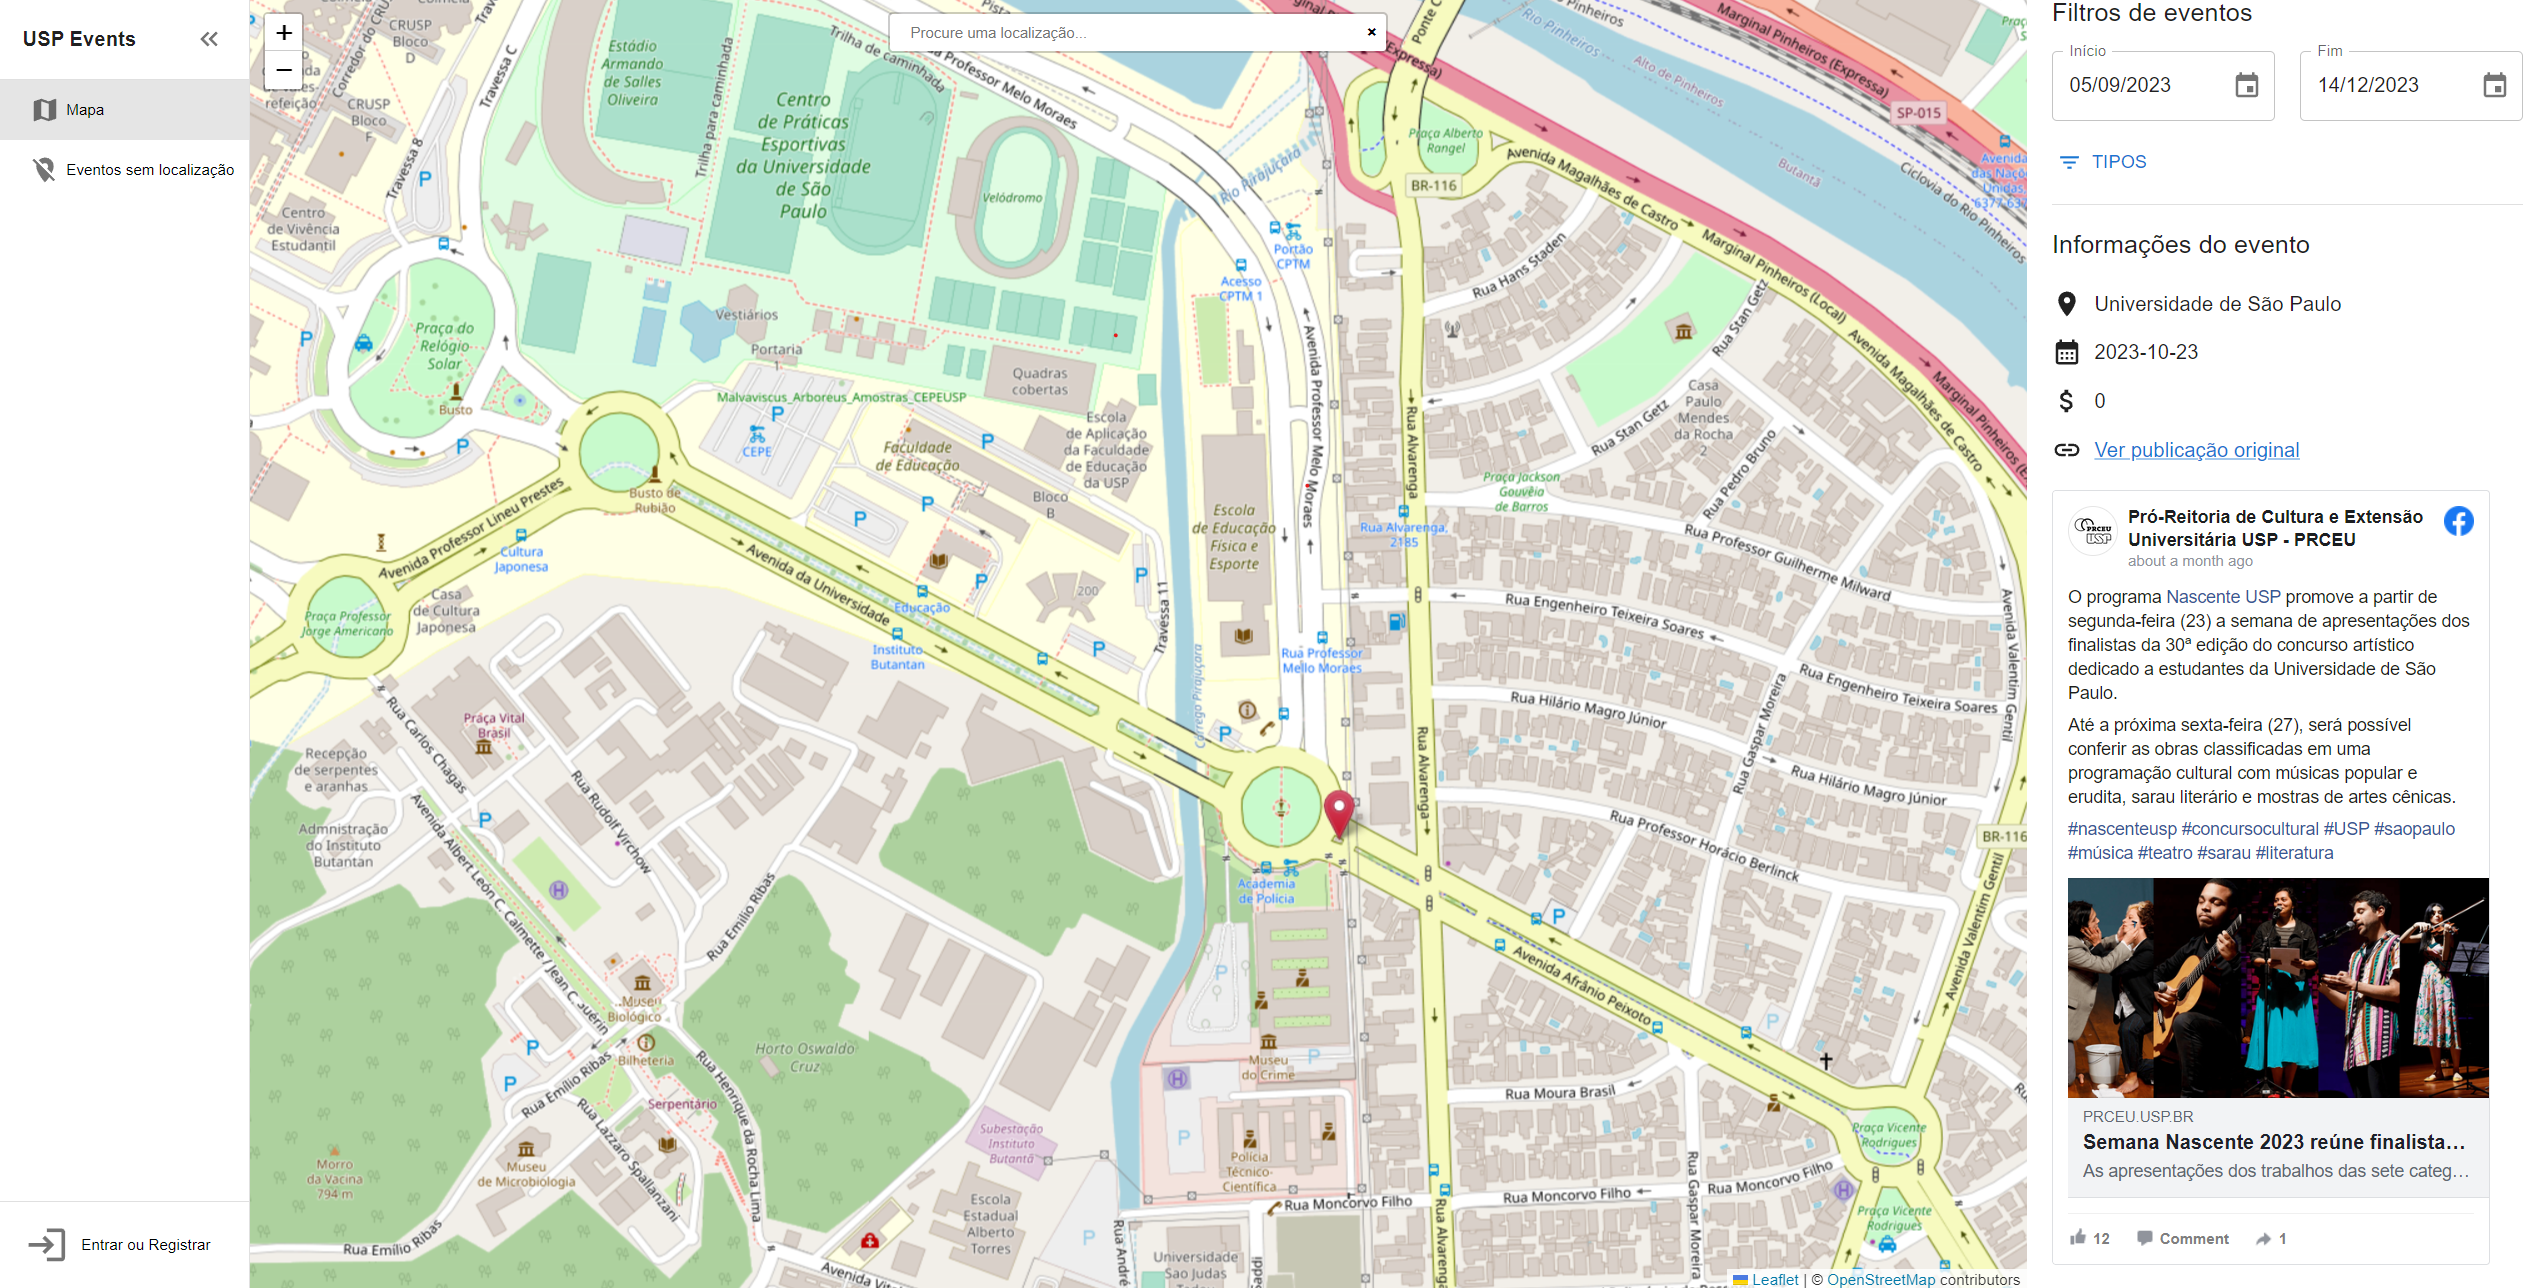
\includegraphics[width=1\textwidth]{figuras/pagina_inicial.png}
    \caption{Página principal do sistema}
\end{figure}

Nela, é possível clicar na localização de eventos disponíveis no mapa. Isso dá
acesso às informações mais granulares sobre eles, como a localização, a data do
evento, o preço de entrada caso exista e um \textit{link} para a sua postagem
original.

No canto superior direito da página, o usuário pode filtrar o período no qual
deseja ver eventos disponíveis e o tipo deles, como eventos culturais e
esportivos.

\begin{multicols}{2}
    \centering
    \vspace*{\fill}
    
\includegraphics[width=.7\linewidth]{figuras/detalhes_eventos.png}
    \captionof{figure}{Detalhes de um evento}
    \vspace*{\fill}

    \columnbreak

    \vspace*{\fill}
    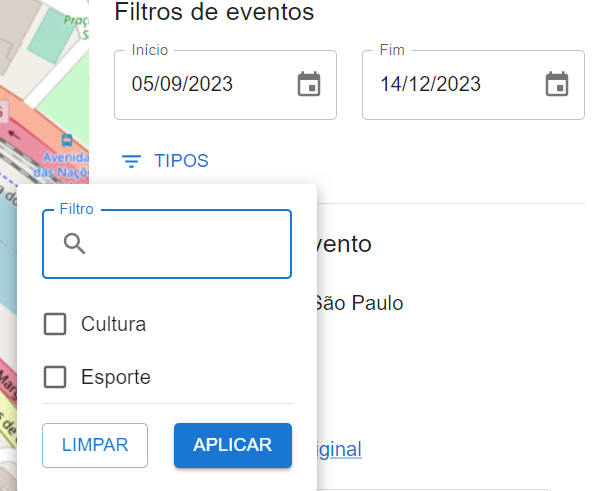
\includegraphics[width=.99\linewidth]{figuras/filtro_eventos.png}
    \captionof{figure}{Filtros de eventos}
    \vspace*{\fill}
\end{multicols}

O primeiro passo necessário para criação do sistema e alimentação desta página
com os dados necessários foi o processo de \textit{webscraping} ou raspagem de
dados. Como foi brevemente descrito no capítulo 2, a plataforma obtém dados de
eventos a partir da aquisição e processamento de textos encontrados nas
postagens em redes sociais.

Para tanto, criou-se um \textit{script} executado a cada 6 horas que busca em
páginas do \textit{facebook} e \textit{instagram} pelos textos das últimas 5
postagens de cada uma delas. Em seguida, eles são encaminhados para uma
ferramenta oferecida pelo \textit{website} \textit{Hugginface chatbot}, no qual
solicita-se que o texto seja processado em busca das informações necessárias
para estruturar um possível evento dentro da plataforma.

\begin{figure}[h]
    \centering
    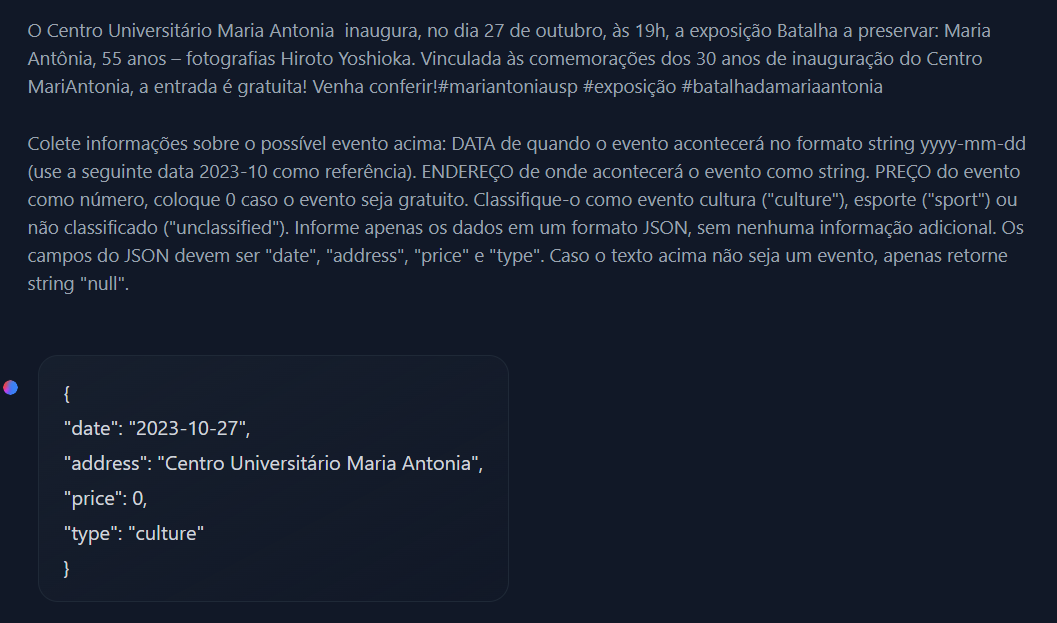
\includegraphics[width=1\textwidth]{figuras/huggingface-chatbot.png}
    \caption{Processamento de um possível evento}
\end{figure}

O \textit{Hugginface chatbot} é basicamente uma plataforma que te permite
interagir com diferentes modelos de \ac{IA} generativa capazes de responder
perguntas gerais ou executar tarefas requisitadas. Eles foram treinados para
entender e gerar textos semelhantes a seres humanos.

Finalizado o processamento textual pelo \textit{chatbot}, o próximo passo é
encontrar a geolocalização com latitude e longitude do evento. Utilizou-se o
serviço gratuito de geocodificação chamado Nominatim para isso, no qual é feita
uma requisição via \acs{API} de um endereço e a saída é a sua respectiva
geolocalização.

Finalmente, caso a maioria das informações sejam encontradas, é possível criar
um evento que é salvo no banco de dados para consumo pelos usuários da
plataforma.

Durante esse processo, surgiram diversos empecilhos e decisões de projeto
pertinentes que serão discutidos a seguir.

\subsection{\textbf{Raspagem de dados}}

Como mencionado no capítulo 2, um dos grandes problemas de realizar a raspagem
de dados via alguma biblioteca externa em mídias sociais é a suspensão
temporária na utilização da aplicação devido a alguma infração nos termos de
uso, mesmo que as páginas sejam abertas ao público.

Esse problema foi contornado temporariamente utilizando a ferramenta Selenium
para simular o uso por um usuário comum e salvar a sessão do navegador. Nesses
\textit{sites}, é comum que precise de uma conta para acessar o seu conteúdo,
mas conectar-se toda vez que executar o processo de \textit{webscraping} não é
o ideal. Por isso que é interessante utilizar algum método para manter a sessão
da conta salva para futuras raspagens de dados.

Um desafio adicional nesta etapa é referente às potenciais mudanças de design
ou funcionalidades nos \textit{websites}. Ao longo do desenvolvimento do
projeto, diversas modificações foram implementadas nas suas estruturas HTML,
deixando o processo de raspagem de dados desatualizado. Consequentemente, todo
o processamento textual ficava comprometido, demandando um tempo considerável
para identificação e correção dos erros. Infelizmente, não existe um método
simples para contornar esse tipo de problema, o que torna esse processo
particularmente tedioso.

\subsection{Processamento de informações}
\label{sec:infoProcessing}

Alguns pontos importantes a se discutir para que o processamento textual fosse
possível são: processo custoso e demorado, escolha do modelo de \acs{IA}
generativa; instruções para guiar o modelo na extração de informações.

A ideia inicial era que o processamento dos textos como descrito anteriormente
fosse realizado em tempo de execução. O que significa que ele executaria a cada
chamada de \acs{API} que o usuário fizesse para requisitar possíveis eventos na
plataforma. Isso logo foi considerado inviável, já que todo o procedimento é
demorado e esse tempo escala à medida que mais textos são processados. A
desvantagem considerada é o atraso de 6 horas de escrita no sistema caso uma
nova postagem seja feita de um evento nas redes sociais.

O alto consumo computacional nesse processo também fez com que se optasse
deixá-lo a encargo de um terceiro, no caso o \textit{Huggingface chatbot}. O
servidor utilizado para hospedar a plataforma dispõe apenas de 4 núcleos de uma
CPU ARM de propósito geral, o que não é ideal para esse caso de uso. Nessas
condições, utilizando o modelo de \acs{IA} generativa
\href{https://huggingface.co/TheBloke/Llama-2-13B-chat-GGUF}{Llama-2}
recentemente disponibilizado pela empresa Meta, foi possível processar um texto
de um evento em aproximadamente 15 minutos e meio. Conforme mais postagens são
analisadas, o tempo gasto se torna absurdo em um cenário normal de uso da
plataforma, enquanto o \textit{chatbot} utilizado é consideravelmente mais
rápido. Porém, essa escolha torna essa etapa dependente de um serviço externo,
o que dificulta a manutenção já que podem ocorrer quebras de contrato
inesperadas ou indisponibilidade do mesmo por certo período, impactando
diretamente nas operações do projeto.

\begin{figure}[h]
    \centering
    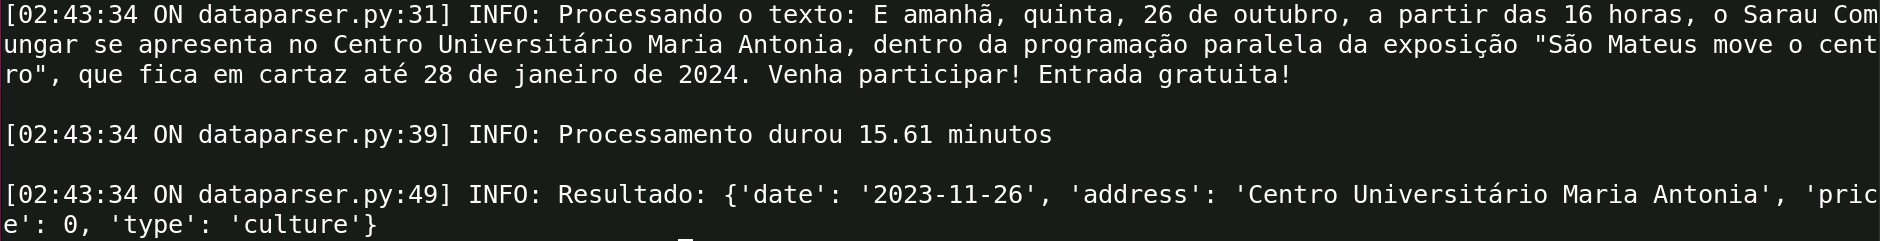
\includegraphics[width=1\textwidth]{figuras/llama_2_local.png}
    \caption{Processamento textual no servidor}
\end{figure}

\begin{figure}[h]
    \centering
    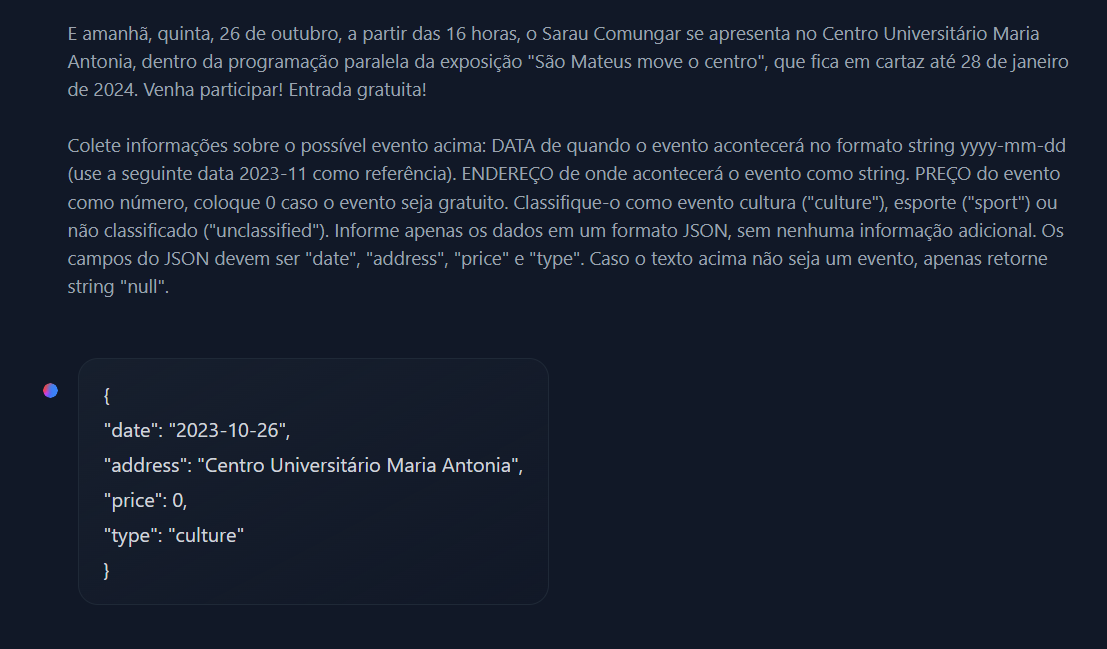
\includegraphics[width=0.6\textwidth]{figuras/huggingface-chatbot2.png}
    \caption{Processamento textual via \textit{Huggingface chatbot}}
\end{figure}

O \textit{chatbot} permite interagir com 5 modelos de código aberto diferentes
até o momento. Dentre eles, está o anteriormente mencionado
\href{https://ai.meta.com/llama/}{Llama-2}, o recente
\href{https://github.com/imoneoi/openchat}{OpenChat 3.5} e o utilizado
\href{https://mistral.ai/news/announcing-mistral-7b/}{Mistral 7B}. A decisão da
escolha do modelo foi feita a partir da qualidade geral das informações
extraídas. No final, observou-se que o \textit{Mistral 7B} apresentou maior
acurácia ao executar a instrução fornecida em comparação com os demais,
principalmente na tarefa de julgar se o texto processado corresponde a um
possível evento ou não.

\begin{multicols}{2}
    \centering
    \vspace*{\fill}
    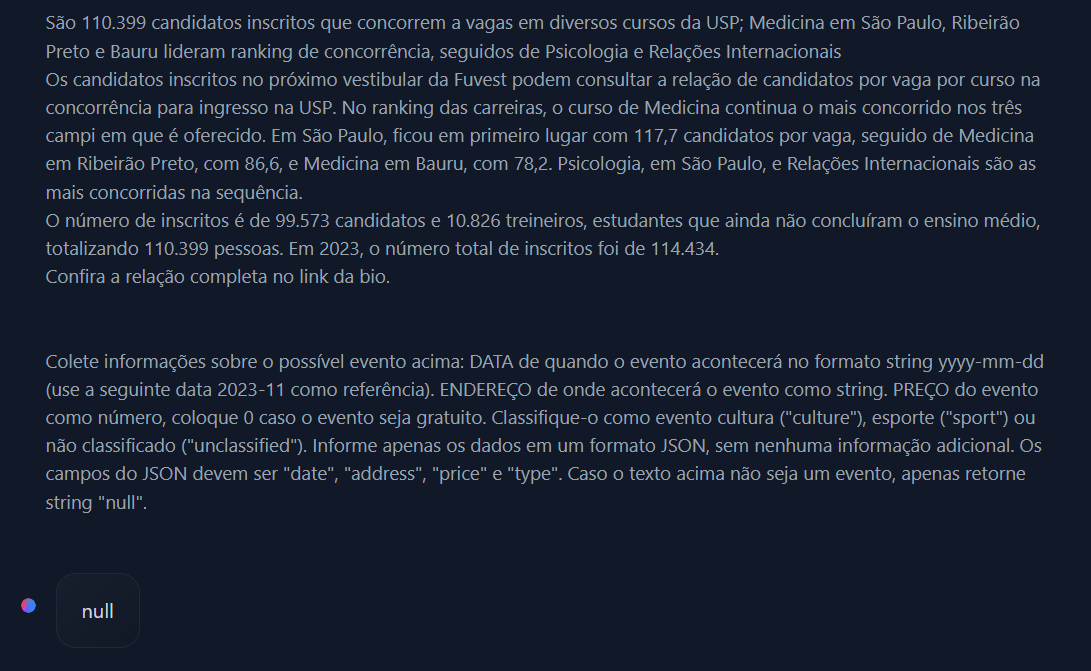
\includegraphics[width=1\linewidth]{figuras/huggingface-not-event.png}
    \captionof{figure}{Processamento textual de um não evento pelo \textit{Mistral 7B}}
    \vspace*{\fill}

    \columnbreak

    \vspace*{\fill}
    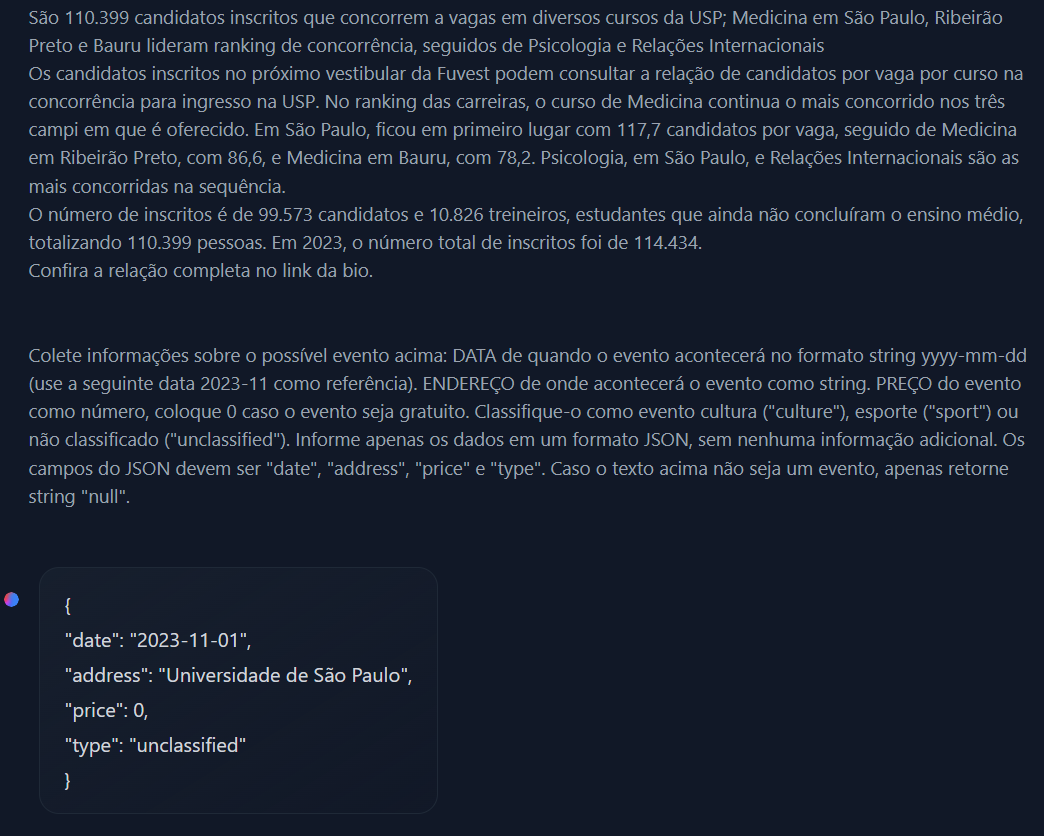
\includegraphics[width=1\linewidth]{figuras/huggingface-not-event-2.png}
    \captionof{figure}{Processamento textual de um não evento pelo \textit{Llama-2}}
    \vspace*{\fill}
\end{multicols}

É importante ressaltar que esses modelos de \acs{IA} generativa foram utilizados com configurações padrão, sem quaisquer mudanças em possíveis parâmetros que pudessem melhorar a qualidade do resultado da tarefa, dado que o \textit{Huggingface chatbot} não oferece essa opção e essa etapa não é o foco do projeto em si, mas sim a construção da plataforma de ponta a ponta.

Além da escolha do modelo, o modo como a instrução é estruturada para que ele
execute a tarefa também interfere diretamente na qualidade dos resultados
obtidos. O processo de construção eficaz dessas instruções direcionadas para
que a \acs{IA} retorne um resultado mais preciso está sendo recentemente
denominada de Engenharia de \textit{Prompts}.

\begin{figure}[h]
    \centering
    \noindent\fbox{
        \parbox{0.9\textwidth}{
            Colete informações sobre o possível evento acima: DATA de quando o evento acontecerá no formato string yyyy-mm-dd (use a seguinte data 2023-11 como referência). ENDEREÇO de onde acontecerá o evento como string. PREÇO do evento como número, coloque 0 caso o evento seja gratuito. Classifique-o como evento cultura ("culture"), esporte ("sport") ou não classificado ("unclassified"). Informe apenas os dados em um formato JSON, sem nenhuma informação adicional. Os campos do JSON devem ser "date", "address", "price" e "type". Caso o texto acima não seja um evento, apenas retorne string "null".
        }
    }
    \caption{Instruções para extração de informações do evento}
\end{figure}

O texto acima corresponde às instruções ou \textit{prompt} utilizado para
extração das informações desejadas. Algumas boas práticas compiladas por
\cite{techtarget2023} foram seguidas no ramo de Engenharia de \textit{Prompts}:

\begin{itemize}
    \item \textbf{Especificidade:} Ao definir exatamente quais informações devem ser buscadas, no caso a data, o endereço, o preço e o tipo de evento, é possível restringir a gama de possíveis respostas e aumentar a probabilidade do modelo produzir a saída desejada.

    \item \textbf{Uso de exemplos:} É provável que o texto não apresente uma data completa do evento, como por exemplo \textit{"No dia 08, a apresentação artística acontecerá..."}. Fornecendo uma data de referência pode ajudar o modelo a entregar uma data inteira que se espera na saída. O mesmo serve para os demais campos, em que se informa o formato do tipo do evento e preço.

    \item \textbf{Formato de saída claramente definido:} Especificar que a informação deve ser retornada em formato JSON foi essencial para que se pudesse interpretá-lo programaticamente posteriormente.
\end{itemize}

Porém, é extremamente importante destacar que o modelo ainda comete muito mais
erros do que acertos, portanto as informações disponibilizadas dentro da
plataforma devem ser usadas com cautela.

\subsection{Código aberto}

A natureza acadêmica da plataforma e a escassez de recursos monetários fizeram
com que fosse claro a preferência pelo uso de tecnologias de código aberto.
Essa escolha, embora alinhada com os princípios de transparência e colaboração
da comunidade acadêmica, não esteve isenta de desafios durante o
desenvolvimento do projeto.

Inicialmente, o processo de geocodificação necessário para adquirir a
geolocalização dos eventos foi feito por meio da \acs{API} do Google Maps, por
conta de sua velocidade e principalmente sua precisão. O Nominatim, por ser uma
solução de código aberto baseada em dados do OpenStreetMap, apresentou
limitações em termos de acurácia na maioria dos casos.

A principal questão que surgiu foi a diferença na abrangência dos dados
geoespaciais entre as duas opções. Enquanto o Google Maps possui uma extensa
base de dados, alimentada por fontes diversas e frequentemente atualizada, o
Nominatim depende das contribuições da comunidade OpenStreetMap, o que pode
resultar em informações menos abrangentes e atualizadas.

\section{Eventos sem localização}

Uma das informações mais importantes contidas em um evento é a sua localização
ou endereço, haja vista que é a partir dela que é possível realizar a busca da
geolocalização e, em consequência, exibir o local do evento no mapa.

Entretanto, durante a etapa de processamento dos eventos, assim como destacamos
no tópico \nameref{sec:infoProcessing}, existem momentos em que o modelo não é
capaz de obter corretamente as coordenadas referentes ao evento, seja por um
erro do próprio modelo em identificar o endereço, ou por uma busca incorreta
das coordenadas correspondentes mesmo que o dado tenha sido encontrado
corretamente, ou até mesmo porque o texto analisado não contém essa informação
de maneira explícita. Independentemente do motivo da falha, neste cenário o
sistema não consegue exibir na página principal estes eventos processados.

\begin{figure}[h]
    \centering
    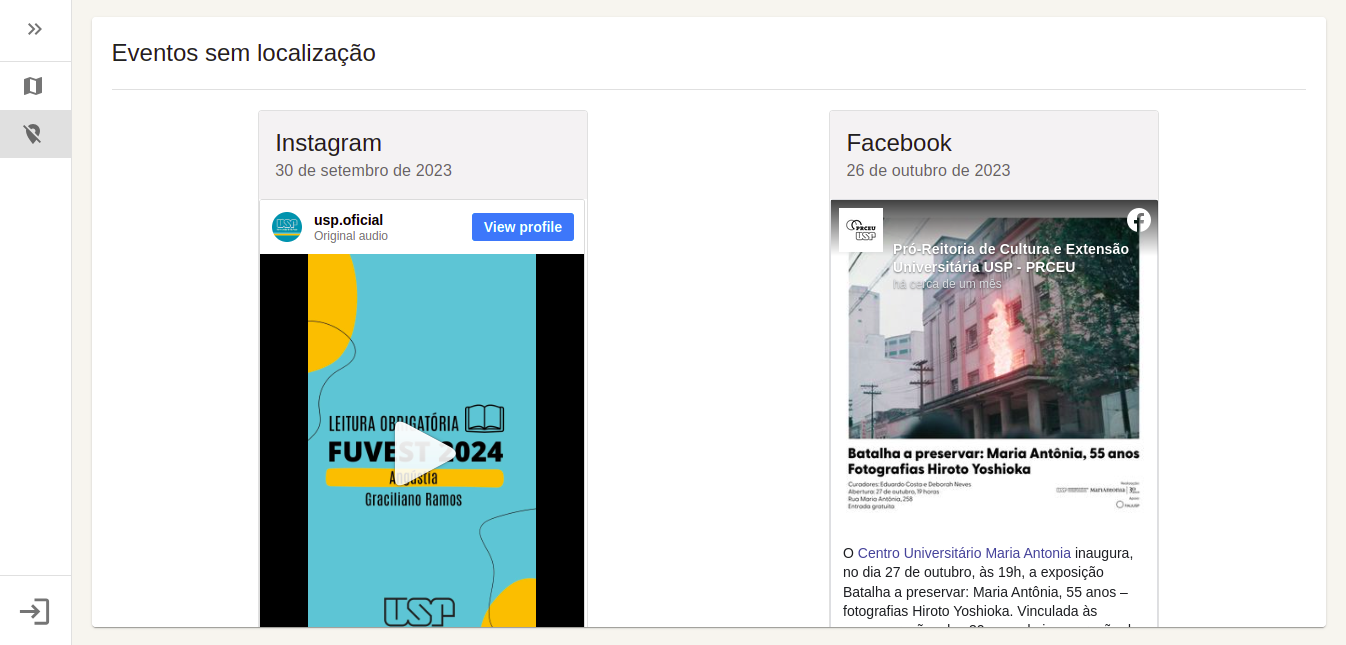
\includegraphics[width=1\textwidth]{figuras/locationlessPage.png}
    \caption{Paǵina de eventos sem localização}
\end{figure}

A página de eventos de localização foi idealizada com o intuito de reunir os
eventos dentro do sistema mesmo com a menor quantidade possível de informações
obtidas a partir do modelo. Esta aba, pode ser acessada através do item na
barra lateral, logo abaixo do mapa.

Devido ao seu design simples, os problemas enfrentados nesta etapa estavam um
pouco mais relacionados com questões mais globais do projeto. O maior problema
esteve relacionado com a maneira em que a identificação de eventos diferentes
era feito dentro do banco de dados. Isso porque a princípio, acreditava-se que
o \textit{link} de cada um dos \textit{posts} seriam distintos entre si, o que
possibilitaria uma fácil diferenciação entre eles. Porém, algumas vezes, os
endereços dos \textit{posts} se alteravam entre execuções de \textit{scraping}
de dados, fazendo com que o sistema interpretasse erroneamente como postagens diferentes,
consequentemente, criando eventos duplicados. Este ponto acabou sendo bem
evidenciado dentro da página de eventos sem localização, como ilustrado na
figura 5.11.

\begin{figure}[h]
    \centering
    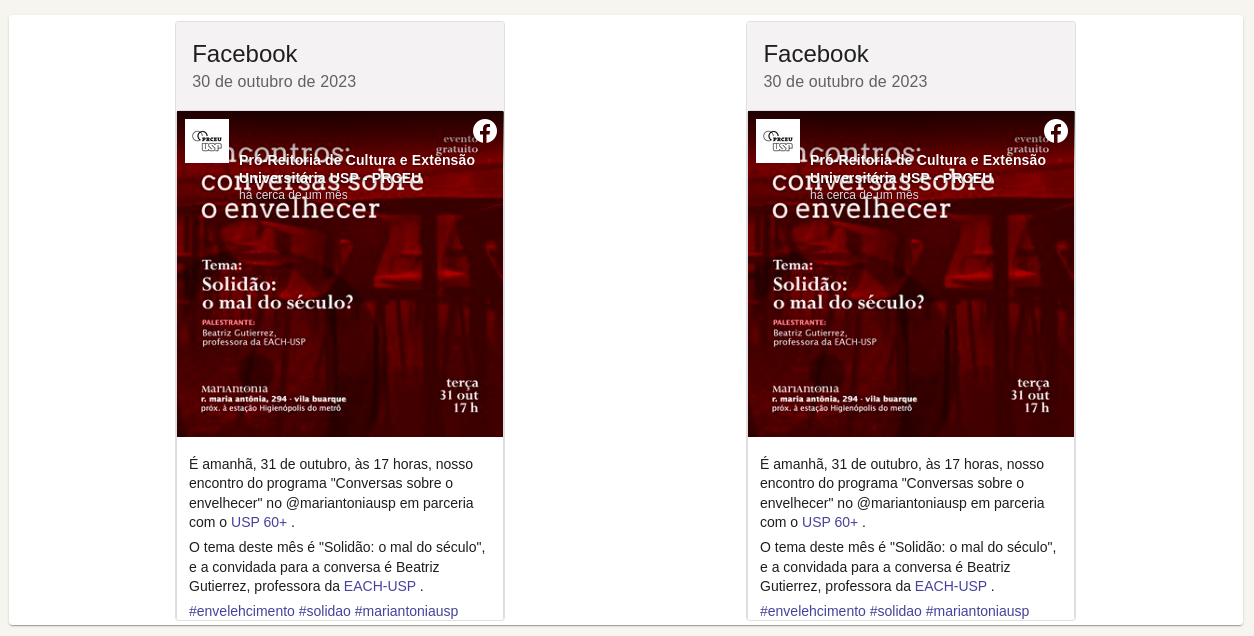
\includegraphics[width=1\textwidth]{figuras/duplicatedEvents.png}
    \caption{Eventos duplicados}
\end{figure}

A maneira para contornar este tipo de problema foi alterar o modo como estes
eventos eram construídos, já que a identificação era feita a partir de um
\textit{hash} que se baseava no \textit{link} para sua construção. Dessa forma,
ao esbarrar no problema de mesmos eventos possuírem endereços distintos em
alguns momentos, foi abordada uma estratégia para considerar, tanto todo o
conteúdo do texto do \textit{post} quanto a sua rede social de origem, para a
construção do \textit{hash} identificador do evento.

\section{Controle de usuários}

O sistema permite que novos usuários acessem e interajam com a plataforma de
forma simples e direta sem qualquer necessidade de cadastro prévio, dessa
forma, como citado na seção inicial deste capítulo, ao navegar pela aplicação,
é possível buscar e filtrar diferentes eventos que estejam próximos de
acontecer. Entretanto, o principal intuito do projeto era deixar o sistema
personalizável e adaptável o máximo possível a partir da inserção de páginas de
interesse do usuário, esta funcionalidade será descrita com mais detalhes na
próxima seção.

\begin{figure}[h]
    \centering
    
\includegraphics[scale=.8]{figuras/loginButton.png}
    \caption{Botão para abrir janela de cadastro ou \textit{login}}
\end{figure}

Por tal motivo, o processo de registro e \textit{login} de usuários é essencial
para que seja possível manter controle das preferências de cada usuário
separadamente. A opção de se registrar ou entrar como um usuário se encontra no
canto inferior esquerdo da tela. Ao clicar neste botão, uma nova janela com
duas abas é aberta, sendo uma destinada para a entrada de usuários já
cadastrados, e a outra, para cadastro de novos usuários no sistema.

Estes formulários contém campos necessários para a criação de um registro de
usuário, como nome de usuário e senha por exemplo, esta última que é armazenada
de forma criptografada no banco de dados. Após o preenchimento das informações,
o sistema realiza uma chamada \acs{HTTP} para o \textit{back-end} para
armazenamento das informações na plataforma.

\begin{multicols}{2}
    \centering
    \vspace*{\fill}
    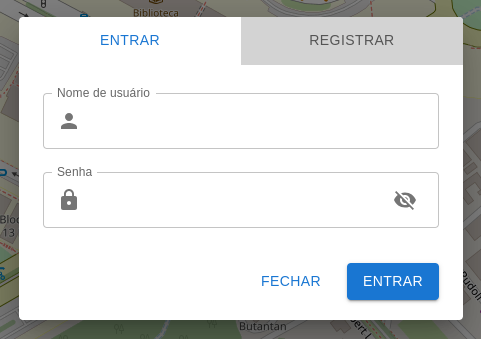
\includegraphics[width=.9\linewidth]{figuras/loginModal.png}
    \captionof{figure}{Janela de \textit{login} de usuários}
    \vspace*{\fill}

    \columnbreak

    \vspace*{\fill}
    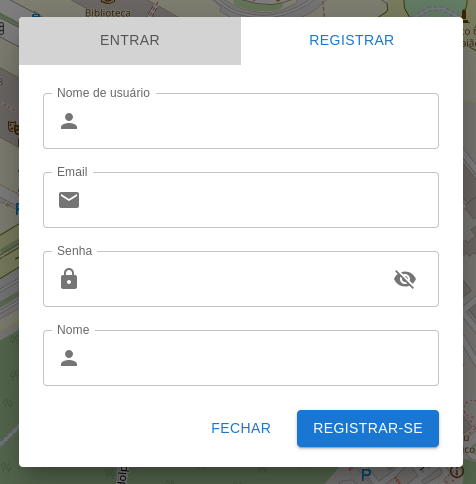
\includegraphics[width=.9\linewidth]{figuras/registrationModal.png}
    \captionof{figure}{Janela de cadastro de novo usuário}
    \vspace*{\fill}
\end{multicols}

\section{Cadastro de páginas}

Após o processo de registro e \textit{login}, o sistema possibilita que os
usuários cadastrem novas páginas que sejam de sua preferência e de onde
gostariam que fossem obtidas as informações necessárias para construção dos
eventos que serão mostrados na tela principal.

\begin{figure}[h]
    \centering
    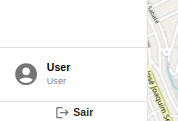
\includegraphics[scale=.8]{figuras/userArea.png}
    \caption{Botão de acesso à área do usuário}
\end{figure}

Esta funcionalidade pode ser acessada através do botão na barra lateral
contendo o ícone de identificação e o nome do usuário logado, como mostra na
figura acima. Com isso, o usuário é redirecionado à página de configurações.

Inicialmente esta página se encontra vazia, apenas com um esqueleto de tabela e
um botão para cadastrar novas páginas na parte superior direita. Ao clicar
neste botão, será aberto um formulário onde o usuário será capaz de registrar
suas páginas de preferência a partir de onde deseja que seus eventos sejam
obtidos.

\begin{figure}[h]
    \centering
    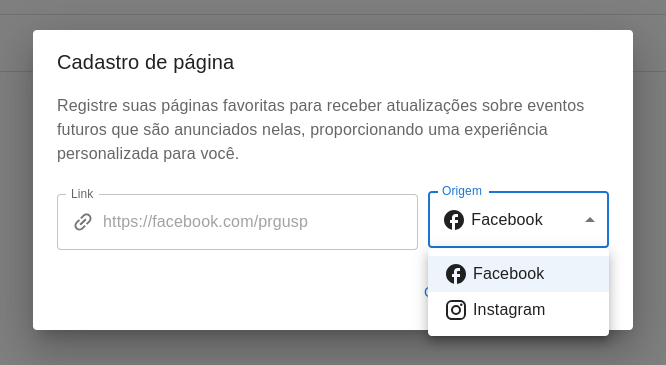
\includegraphics[scale=.5]{figuras/webpageRegisterModal.png}
    \caption{Formulário de registro de \textit{webpages}}
\end{figure}

Neste formulário, existe a possibilidade de cadastrar páginas tanto do
\textit{Facebook} quanto do \textit{Instagram}. O sistema faz uma verificação
através de expressões regulares para garantir que o texto inserido esteja no
formato de uma página \textit{web} e que pertença à rede social escolhida na
seleção.

A visualização das páginas é possível apenas para os usuários que fizeram o seu
registro, ou seja, cada página cadastrada é única para cada usuário diferente,
o que torna a experiência de cada pessoa personalizável aos seus próprios
gostos e interesses. Vale ressaltar o fato de que apesar da unicidade das
páginas para cada usuário, ainda é possível que dois usuários diferentes
insiram uma mesma página nas suas preferências, por isso, a relação
\nameref{sec:WebPageUsers} criada no banco de dados é importante, já que é
através dela que a associação de um usuário à uma \textit{webpage} criada por
ele pode ser identificada.

Ao cadastrar novas páginas, é iniciada a construção de uma lista na tabela que
fica disponível para visualização exclusiva do usuário, ou seja, apenas o
responsável pelo cadastro da página em questão consegue visualizar seu registro
na tabela.

\begin{figure}[h]
    \centering
    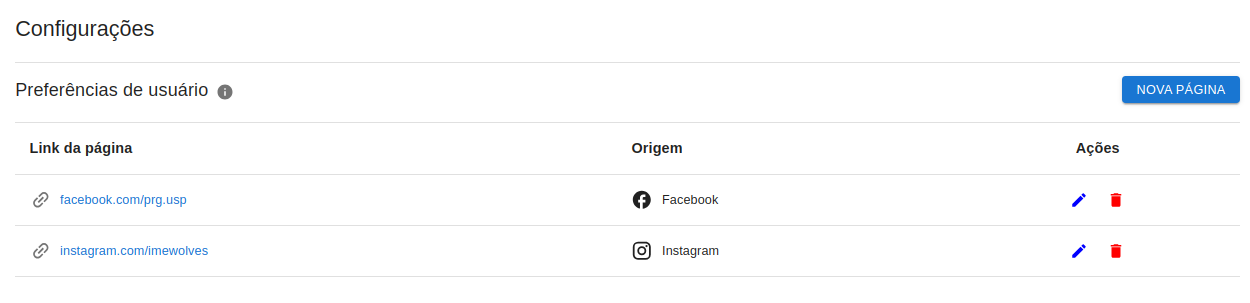
\includegraphics[width=1\textwidth]{figuras/webpagesTable.png}
    \caption{Aparência da página com \textit{webpages} cadastradas}
\end{figure}

A partir do cadastro de suas páginas de preferência, os usuários são capazes de
realizar a edição ou a remoção das informações que não tenham mais interesse
através dos ícones de ação localizado em cada uma das linhas da tabela. Essas
ações sobre cada uma das \textit{webpages} são controladas por meio de
\acp{API} feitas no \textit{back-end} do projeto, estas necessitam que um
\textit{token} de autorização seja passado nas requisições \acs{HTTP} para
diferenciar cada uma das páginas e cada um dos usuários que as cadastraram.

\begin{figure}[h]
    \centering
    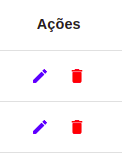
\includegraphics[scale=.5]{figuras/webpageActions.png}
    \caption{Ícones de ação de \textit{webpages}}
\end{figure}

Apesar do desenvolvimento desta etapa ter sido desafiador, grande parte dos
problemas enfrentados e as decisões tomadas para contorná-los já foram
destacados em outras seções. Na seção \nameref{sec:EventsSampling}, por
exemplo, é citado que um dos principais empecilhos enfrentados no projeto foi a
dificuldade em se obter os dados através do processamento em tempo de execução,
e este problema é realçado dentro da funcionalidade descrita nos parágrafos
anteriores, já que, mesmo o sistema permitindo que o registro e alteração das
páginas possa ser feito à qualquer momento, essas mudanças serão perceptíveis,
em termos da visualização dos eventos pelo usuário, em até 6 horas no pior
caso, já que este foi o intervalo escolhido entre cada execução automatizada do
processo de obter os eventos.

\subsection{Controle de páginas para usuários diferentes}

O maior empecilho enfrentado nesta seção, foi em relação ao controle de
\textit{webpages} iguais para diferentes usuários. Como descrito nesta seção, o
sistema permite que uma mesma página seja cadastrada durante interações
distintas de diferentes usuários. Entretanto, neste cenário, torna-se
necessário que o controle para ambas as pontas sejam independentes entre si, ou
seja, mudanças realizadas por um usuário, como uma edição ou uma deleção da
\textit{webpage} por exemplo, devem ser refletidas apenas para quem as fez. O
problema relacionado à este ponto se deu pela maneira como as \acp{API} estavam
construídas, de forma que este comportamento ideal não estava sendo mantido. A
princípio quando dois usuários possuíam um cadastro da mesma página e um deles
realizava alguma ação sobre ela, a mudança era refletida na outra ponta
indevidamente.

O problema ocorria devido ao modo que as \acp{API} interagiam com os dados do
banco para poder realizar as ações solicitadas pelo usuário, isso porque, mesmo
com a existência da relação \nameref{sec:WebPageUsers}, a ação era realizada
sobre a própria \textit{webpage} ao invés de agir apenas sobre o registro da
ligação intermediária entre o usuário que realizou a ação e a página, dessa
forma, do ponto de vista do usuário que teve seu registro alterado
incorretamente, sua referência era mantida, porém a entidade referenciada havia
sido alterada o que causava a mudança indevida do seu registro.

O processo de correção deste problema levou à criação de algumas tarefas no
quadro de atividades para que fossem priorizados, já que era um comportamento
que afetaria a qualidade do sistema em produção e, apesar de a solução parecer
simples, a implementação trouxe alguns empecilhos de implementação,
principalmente causados pela falta de experiência com o \textit{framework}
utilizado no controle das \acp{API}. Além disto, a correção para as ações de
deleção e edição também diferiam entre si, sendo necessário uma abordagem de
reparo distinto para cada método.

